%!TEX root = ../main.tex
%%%%%%%%%%%%%%%%%%%%%%%%%%%%%%%%%%
% Links:
%
% Difficulty: Companies: 
%%%%%%%%%%%%%%%%%%%%%%%%%%%%%%%%%%

\chapter{Sudoku}
\label{ch:sudoku}
\section*{Introduction}
The game of \textit{Sudoku}\footnote{The literal meaning of \quotes{Su-doku} in Japanese is "the number
that is single".} has become hugely popular in the last 20 years to There are now countless websites and magazines dedicated to these mathematical-logic-based
number-placement puzzles.  The objective of this is to fill a nine-by-nine (9x9) grid (subdivided in
$3\times3$ subgrids) with digits so that each:
\begin{itemize}[]
	\item \textbf{row},
	\item \textbf{column},
	\item $3\times3$ \textbf{subsquare section}
\end{itemize}
contains a number between $1$ and $9$, with the constraint that each number can appear only once in
each section. The puzzle is given as a incomplete grid where only some of the cells are filled.

This chapter describes how to write a very basic and simple sudoku solver based on backtracking that
can be implemented fast enough for a programming interview. Having played this puzzle before
might help during the interview but it is not essential as the rules are easy enough to
understand in a few minutes.

%\begin{figure}
	%\label{fig:sudoku:example}
	%\centering
	%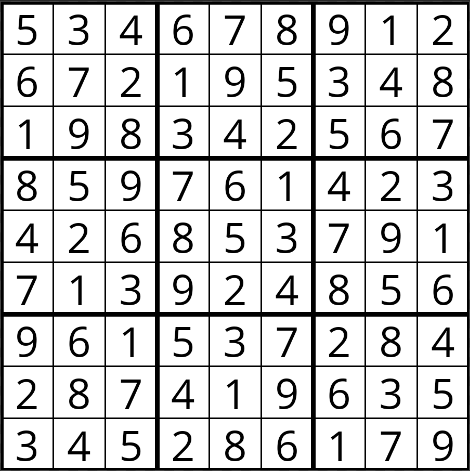
\includegraphics[width=\textwidth]{sources/sudoku/images/sudoku-example}
	%\caption{Example of solved sudoku.}
%\end{figure}

\section{Problem statement}
\begin{exercise}
Write a function that takes as an input a sudoku grid and returns its solution. The input sudoku
grid is given as a string of length $81$ representing the grid in a row-major manner\footnote{In
row-major order, the rows of the grid are stored next to each other in the string.} where empty
cells are represented by the character '0'.
\end{exercise}


\begin{example}
	\hfill \\
	Given the input string
	\tiny{\texttt{\quotes{000060280709001000860320074900040510007190340003006002002970000300800905500000021}}}
	{\normalsize the function returns}
	{\tiny\texttt{\quotes{431567289729481653865329174986243517257198346143756892612975438374812965598634721}}}
	\normalsize. See Table \ref{tab:sudoku:grid_solution} for a 2D-grid representation.
	
	\begin{table}[]
	\centering
		\begin{tabular}{|l|l|}
			\hline
			Input & Solution \\ \hline
			\texttt{
				\begin{tabular}[c]{@{}l@{}}
					0 0 4 3 0 0 2 0 9 \\ 
					0 0 5 0 0 9 0 0 1 \\ 
					0 7 0 0 6 0 0 4	3 \\
					0 0 6 0 0 2 0 8 7 \\
					1 9 0 0 0 7 4 0 0 \\ 
					0 5 0 0 8 3 0 0 0 \\ 
					6 0 0 0 0 0 1 0 5 \\ 
					0 0 3 5 0 8 6 9 0 \\ 
					0 4 2 9 1 0 3 0 0
				\end{tabular}
			} & 
			\texttt{
				\begin{tabular}[c]{@{}l@{}}
					8 6 4 3 7 1 2 5 9 \\
					3 2 5 8 4 9 7 6 1 \\ 
					9 7 1 2 6 5 8 4 3 \\ 
					4 3 6 1 9 2 5 8 7 \\
					1 9 8 6 5 7 4 3 2 \\ 
					2 5 7 4 8 3 9 1 6 \\
					6 8 9 7 3 4 1 2 5 \\
					7 1 3 5 2 8 6 9 4 \\
					5 4 2 9 1 6 3 7	8
				\end{tabular}
			}
			\\ \hline
		\end{tabular}
	\caption[Example of Sudoku (2D) and its solution.]{Example of Sudoku grid (on the left) and its solution (on the right). Note that empty cells are denoted here with the character '0' (zero).}
	\label{tab:sudoku:grid_solution}
	\end{table}
\end{example}


\section{Clarification Questions}

\begin{QandA}
	\item \begin{questionitem} \begin{question} Is the input string guaranteed to only contains numeric characters and be the right size?  \end{question} 	 
    \begin{answered}
		\textit{Yes the string is guaranteed to be encoding a valid sudoku}
	\end{answered} \end{questionitem}	
\end{QandA}

\section{Discussion}
\label{sudoku:sec:discussion}
The general problem of solving a sudoku (of size $n\times m$) is NP-complete\footnote{NP stands for
Non-deterministic Polynomial time. A problem that can be solved in polynomial time (efficiently) by
a non-deterministic turing machine and for which the solution can be efficiently verified to be
correct by a deterministic turing machine. A problem in NP is complete if by solving it you are able
to solve every other problem in NP. This means that an NP-complete problem is at least as hard as
every other problem in NP.} and thus an efficient (polynomial-time) solution is not yet known. The
simple bruteforce algorithm would have to try each available number across all empty cells and
therefore would have a runtime complexity of $O(N^{(N^2)})$, where $N$ is size of the Sudoku puzzle.
For a classic  $9 \times 9$ puzzle $N = 9$ and the number of operations required would be at most $2
\times 10^{77}$ operations to find a solution which would make this approach
impractical. 

In practice the number of operations varies hugely according to the difficulty of the puzzle itself
and especially according to the number of given clues which, in turn, limit the options for each empty
cell. Clues reduce the number of possible states the grid can be  and in which the rules of the
puzzle are not violated. The more clues the are, the higher the number of invalid states. An algorithm can take
advantage of that fact to avoid those invalid states. For example, a $17$-clue puzzle with diagonal symmetry is
one of the hardest to solve due to the large number of candidates and branches\footnote{$17$ clues
has been proven to be the lower-bound for having a puzzle with a \textbf{unique} solution}. 

\subsection{Backtacking}
\label{sudoku:sec:bruteforce}

Backtracking is a good approach to use to solve this problem considering that it
has the following characteristics:
\begin{itemize}
	\item potentially large puzzle-states search space
	\item many \textit{invalid} states we can skip visiting
\end{itemize}
For a more detailed explanation of backtracking see \cite{backtracking}.

In a nutshell the solution proposed in this section works by visiting the empty cells starting from
the first one from the lest, filling it in with a feasible digit (i.e. a digit that does not take the
grid to an invalid state) and then doing the same for every other empty cell. If at
any point there is no available digit for an empty cell then a backtracking step occurs. The
choice for the previous cell is then changed and the whole process repeats until either all the
empty cells are filled (in this case we have a valid solution) or there are no more options for the
first cell (in this case the puzzle has no solution and it is invalid). A backtracking solution
would solve a puzzle by placing the digit '1' in the first empty cell and checking if it is allowed
to be there  (i.e. that no rules are broken). If there are no violations (checking row, column, and box
constraints) then the algorithm advances to the next cell and places a '1' in the next empty cell.
When checking for violations, if it is discovered that the \quotes{1} is not allowed, the value is advanced
to \quotes{2}. If a cell is discovered where none of the 9 digits is allowed, then the algorithm leaves
that cell blank and moves \textbf{back} to the previous cell. The value in that cell is then
incremented by one and the whole process repeats. Clearly, this method will eventually find a
solution if the puzzle is valid because all possible valid states for the grid will be tested. 


Listing \ref{list:sudoku} shows a possible implementation of the backtracking idea described above.
The public interfact of the SudokuSolver class consists only of a constructor
\lstinline[columns=fixed]{SudokuSolver::SudokuSolver(std :: string} taking a a sole input a
\lstinline[columns=fixed]{std::string}, the problem input, and the
\lstinline[columns=fixed]{std::strings SudokuSolver::solve()} function that is responsible for
returning the solution. The constructor is responsible for analyzing the input and storing the indices of all the empty
cells (i.e. the cells the backtracking function is going to try to fill) in a
vector(\lstinline[columns=fixed]{std :: vector < int >blankCells}).

The core implementation function is the \lstinline[columns=fixed]{bool solve\_helper(const int i)}
recursive function that takes as input an integer \lstinline[columns=fixed]{cell} representing the
index of an empty cell in the input string. The base case for this function is when
\lstinline[columns=fixed]{i >= blankCells . size ()} i.e. there are no more empty cells to be filled.
The rest of the function is straightforward because it only consists of a loop trying all
possible numbers for that cell from '1' to '9'. The \lstinline[columns=fixed]{canInsert(char x, int pos)} function is responsible
for deciding whether a character \lstinline[columns=fixed]{x} can be placed in a certain cell
\lstinline[columns=fixed]{pos}. The check is performed by examining whether any of the rules
described above would be broken by having \lstinline[columns=fixed]{x} at cell
\lstinline[columns=fixed]{pos}. If no rules are broken then the function
\lstinline[columns=fixed]{solve_helper} calls itself recursively on the \textbf{next} empty cells
i.e. \lstinline[columns=fixed]{cell+1}. If none of the values tried in the loop yield a valid
solution then the function returns false (no value can be inserted at this location without
violating one or more rules).

Because the input is a linear representation of a grid, which is a 2D structure, and the constraints
of the puzzle are for the 2D portion of the grid itself, the code is further complicated by calculations
that are necessary for the functions \lstinline[columns=fixed]{canInsertInRow},
\lstinline[columns=fixed]{canInsertInCol} and \lstinline[columns=fixed]{canInsertInSquare} to be
able to map the cells belonging to the same row, column or subsquare to the input 1D input string.
The functions \lstinline[columns=fixed]{getRow}, \lstinline[columns=fixed]{getCol},
\lstinline[columns=fixed]{getSubsquare} are used to -  given a index in the 1D input string  - retrieve
the corrensponding row, column and subsquare index in the 2D grid. These functions are used in the
\lstinline[columns=fixed]{canInsertInRow}, \lstinline[columns=fixed]{canInsertInCol} and
\lstinline[columns=fixed]{canInsertInSquare} functions that are responsible for verifying that the
constraints on the row, column and subsquare, respectively, are not violated when we try to insert a
certain value in a cell. In order to do this they need to be able to calculate the indices
of all cells belonging to the same row, columns and subsquare. Specifically:
\begin{itemize}
	\item the \lstinline[columns=fixed]{canInsertInRow} function checks all the cells belonging to
	the same row. Given a row $r$ then all $9$ cells belonging to it have indices in the range
	$[9r,9(r+1)]$(See Figure \ref{fig:sudoku:getRow}).
	\item It becomes more complex when it comes to checking cells in the same column, in the
	function \lstinline[columns=fixed]{canInsertInRow}. The column $c$ to which a cell in the input
	string with index $x$ belongs can be found by using the following formula: $c = x \Mod{9}$. This
	means that the very first cells in the input belonging to column $c$ is located at index $c$ and
	all subsequent cells of the column are distanced $9$ cells from each other. More formally, the
	index for the $k^{th}$ cell of the column in the input string is: $P(k,c) = 9k+c$.
	\item The hardest check is the one for subsquares in the
	\lstinline[columns=fixed]{canInsertInSquare(char x, int s)} function because, in order to check
	whether it is possible to insert the value $x$ in the subsquare $s$,  it has to compare $x$ to all
	the other non-empty cells of the same subsquare. This goal is accomplished in two steps:
	\begin{enumerate}
		\item First, the index of the $F(s)$ top left corner of the subsquare $s$ is calculated  by
		using the following formula: $F(s) = (27 \lfloor \frac{s \rfloor{3}}) + (3\times (s \mod{3}))$.  In
		order to understand the formula, we need first to note that the subsquares are organized
		into $3$ rows each of size $3$ (for a total of 9 subsquares, see Figure \ref{fig:sudoku:}).
		Clearly each subsquare contains $9$ cells, and thus, a full row of subsquares contains
		$3\times9 =27$ cells. $\frac{s}{3}$ is a value representing how many full subsquare rows
		come before $s$. Clearly we can skip all the cells belonging to those subsquares, because
		all cells in them come before $F(s)$. The value $(27 \lfloor \frac{s \rfloor{3}})$ is thus an index
		pointing to a cell at the beginning of the row where $F(s)$ is located. All we need to do
		now is to advance to the correct subsquare in the row and we can do that by looking at the
		position of the subsquare \textbf{in the row} which clearly is $(s \Mod{3})$; $s$ can either
		be either on the left ($(s \Mod{3})=0$), center ($(s \Mod{3})=1$) or on the right side of
		the row ($(s \Mod{3})=2$). Given each subsequare has width of $3$ we can jump to the
		correct location by using $3\times  (s \Mod{3}))$. 
		\item once $F(s)$ is known then is it easy to retrieve the indices of all the cells in the
		subsquare by using the ideas adopted for
		\lstinline[columns=fixed]{canInsertInRow} and \lstinline[columns=fixed]{canInsertInCol}.
	\end{enumerate}
	
\end{itemize}


\lstinputlisting[language=c++, caption={Backtracking solution to the Sudoku problem.},label=list:sudoku]{sources/sudoku/sudoku_solution1.cpp}


\section{Conclusion}


